


\section{Auswertung}
\label{sec:auswertung}

In diesem Kapitel werden die aufgenommenen Messwerte ausgewertet.
\subsection{Der Invertierende-Linearverstärker}
\label{sec:linearverstaerker}
Bei dieser ersten Schaltung wurden für zwei verschiedene Widerstandsverhältnisse Eingangs- und Ausgangsspannung,
$U_a$ und $U_e$, sowie der zeitliche Versatz $\Delta t$ der beiden Signalamplituden vom Oszilloskop abgelesen. 
Zunächst wird dann der reale Verstärkungsfaktor $x$ mithilfe der von \autoref{eq:vfaktor} berechnet und in 
\autoref{fig:linearverstaerker} gegen die Frequenz $f$ des Eingangsignals aufgetragen. Der Phasenverschiebungswinkel
$\phi$ wurde dann über \autoref{eq:phasenverschiebung} errechnet und in \autoref{fig:phasenverschiebung} 
ebenfalls gegen die Frequenz aufgetragen.

\begin{equation}
    \label{eq:vfaktor}
    x=\frac{U_a}{U_e}
\end{equation}

\begin{equation}
    \label{eq:phasenverschiebung}
    \phi=2\pi f \Delta t
\end{equation}
Der theoretische Wert für die Verstärkung ist durch \autoref{eq:thverstaerkung} gegeben und beträgt für
die Widerstandskombination $R_1=\SI[]{1}[]{k\Omega}$, $R_2=\SI[]{100}[]{k\Omega}$, $x_1=100$. Für die 
Widerstandskombination $R_1=\SI[]{1}[]{k\Omega}$, $R_2=\SI[]{10}[]{k\Omega}$, beträgt er $x_2=10$.
\begin{figure}
    \centering
    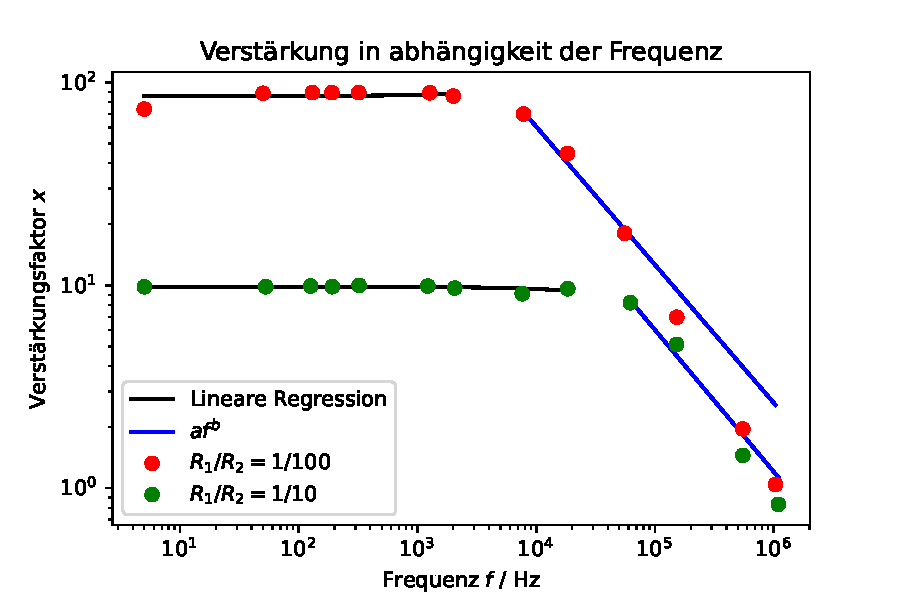
\includegraphics{content/grafiken/verstaerkung.pdf}
    \caption{Verstärkungskurve des als invertierenden Linearverstärker geschalteten Operationsverstärkers nach Eingangsfrequenz.}
    \label{fig:linearverstaerker}
  \end{figure}
  An die konstanten Plateubereiche der Verstärkungskurve wurde je eine Grade nach der Vorschrift $x(f)=af+b$ 
  mit den Parametern:
   \begin{center}
       $a_{1/100} =  0.001\pm 0.003$\\
       $b_{1/100} = 85.819\pm 2.946$\\
       $a_{1/10}  =  0.000\pm 0.000$\\
       $b_{1/10}  = 9.834 \pm 0.095$\\
   \end{center}
 angepasst. Die Steigungen $a_{1/100}$ und $a_{1/10}$ sind vernnachlässigbar klein so das die Verstärkung
 hier als Konstant betrachtet werden kann. An die in der gewählten doppelt-logarithmischen Darstellung
 Funktionsabfälle wurden hingegen Kurven der Vorschrift: 
 \begin{equation}
    \label{eq:exponentialgesetz}
    x=cf^d
 \end{equation}
  angepasst. Daraus folgen die Parameter:
  \begin{center}
    $c_{1/100} = 32076.147  \pm 16619.806$\\
    $d_{1/100} =   -0.681 \pm 0.056$\\
    $c_{1/10} = 18911.087 \pm 21201.677$\\
    $d_{1/10} =   -0.699 \pm 0.099$\\
  \end{center}
  \begin{figure}
    \centering
    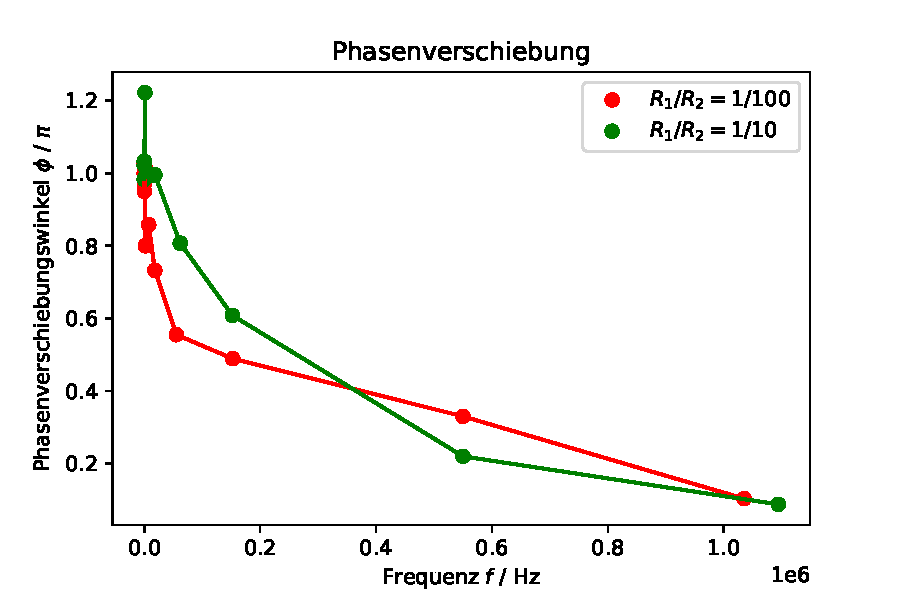
\includegraphics{content/grafiken/phasenverschiebung.pdf}
    \caption{Phasenverschiebung am invertierenden Linearverstärker in Abhängigkeit der Zugangsfrequenz.}
    \label{fig:phasenverschiebung}
  \end{figure}
Der Frequenzabhängige Verlauf des Phasenverschiebungswinkels gleicht dem eines LR-Gliedes. Er beginnt bei kleinen
Freuenzen bei etwa $\pi$ und strebt dann gegen null.
Die Grenzfrequenzen liegen bei  $f_{grenz,1}=9970.01\pm 8436.61$ und $f_{grenz,2}=81931.26\pm 23183.478$ 6.953

\subsection{Der Umkehrintegrator und der invertierender Differenzierer}
\label{sec:umkehrintegrator}
Für den Aufbau des Umkehrintegrators nach \autoref{fig:SPumkehrintegrator} wurde ein Widerstand von 
$R=\SI[]{10}[]{k\Omega}$ und ein Kondensator mit der Kapazität $C=\SI[]{100}[]{nF}$ verwendet. 
Es wurde mit \autoref{eq:vfaktor} erneut der Verstärkungsfaktor berechent und gegen die Frequenz aufgetragen.
Im niedrigen Frequenzbereich wurde eine Kurve nach \autoref{eq:exponentialgesetz} angepasst. Die Parameter 
lauten hier:
\begin{center}
    $c_{Int} =  191.631 \pm 17.526$\\
    $d_{Int} =   -1.006 \pm 0.034$\\
\end{center}
Das Ergebnis ist in \autoref{fig:umkehrintegrator} dargestellt. 

\begin{figure}
    \centering
    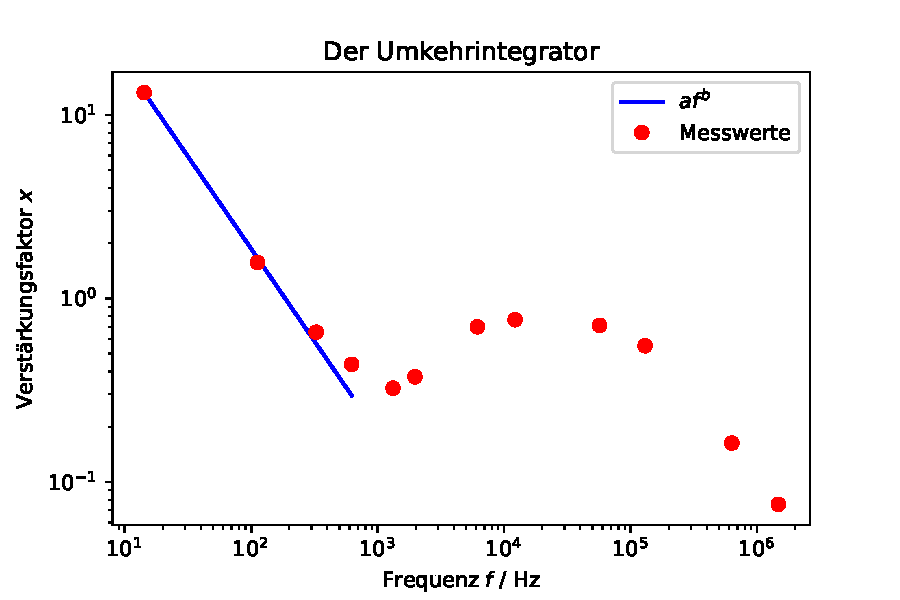
\includegraphics{content/grafiken/umkehrintegrator.pdf}
    \caption{Verstärkungskurve des Umkehrintegrators nach Eingangsfrequenz}
    \label{fig:umkehrintegrator}
  \end{figure}
Im Anschluss daran wurde zunächst ein Sinus-, dann ein Dreiecks- und am Ende ein Rechtecksignal
auf den Eingang der Schaltung gegen und dann das Eingangs- mit dem Ausgangsignal auf dem Oszilloskop 
dargestellt. Die Ergebnisse sind in \autoref{fig:sinusI}, \autoref{fig:dreieckI} und \autoref{fig:rechteckI}
zu sehen.

  \begin{figure}
    \centering
    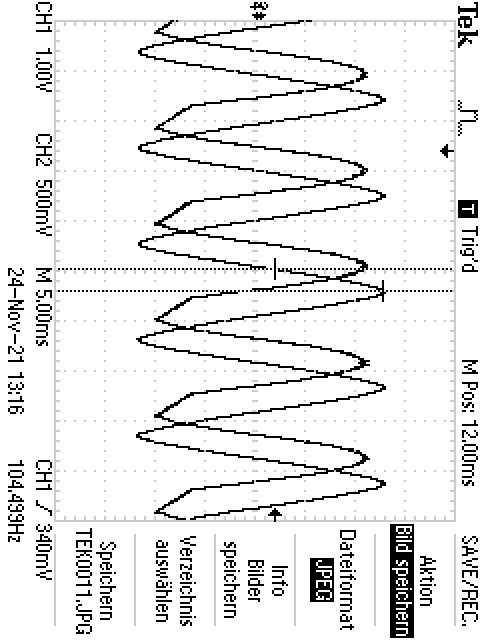
\includegraphics[width=0.3\textwidth,angle=90]{content/grafiken/umkehrIntegrator/TEK0011.JPG}
    \caption{Oszilloskopbeild des Umkehrintegrators bei einer sinusförmigen Eingangsspannung.}
    \label{fig:sinusI}
  \end{figure}
  \begin{figure}
    \centering
    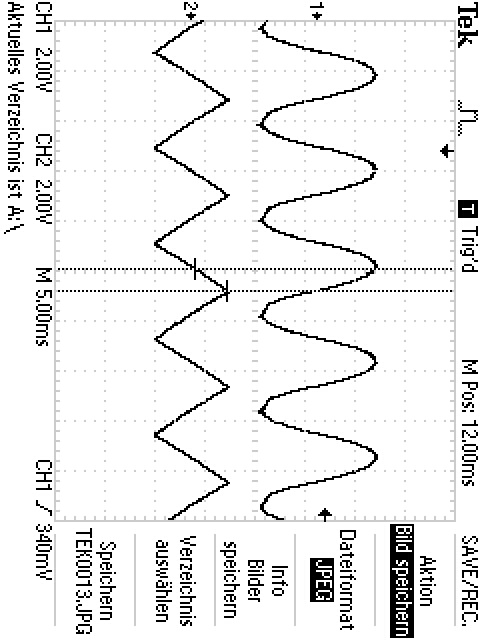
\includegraphics[width=0.3\textwidth,angle=90]{content/grafiken/umkehrIntegrator/TEK0013.JPG}
    \caption{Oszilloskopbeild des Umkehrintegrators bei einer dreieckförmigen Eingangsspannung.}
    \label{fig:dreieckI}
  \end{figure}
  \begin{figure}
    \centering
    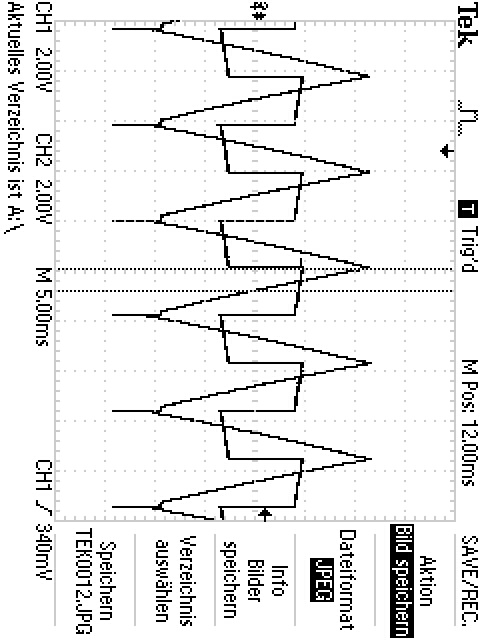
\includegraphics[width=0.3\textwidth,angle=90]{content/grafiken/umkehrIntegrator/TEK0012.JPG}
    \caption{Oszilloskopbeild des Umkehrintegrators bei einer rechteckförmigen Eingangsspannung.}
    \label{fig:rechteckI}
  \end{figure}
\newpage
Beim invertierenden-Differenzierer wurde exakt analog vorgegangen. Die Bauteilwerte des Widerstandes 
und des Kondensators betrugen hier $R=\SI[]{100}[]{k\Omega}$ und $C=\SI[]{22}[]{nF}$. Die nach
\autoref{eq:exponentialgesetz} angepasste Kurve hat die Parameter:
\begin{center}
    $c_{dif} =    0.012 \pm 0.000$\\
    $d_{fif} =    0.981 \pm 0.005$\\
    
\end{center}
und ist im $x$-$f$-Diagramm in \autoref{fig:invdifferenzierer} dargestellt.
Die Oszilloskopbilder für die verschieden förmigen Eingangssignale sind in  \autoref{fig:sinusII},
 \autoref{fig:dreieckII} und \autoref{fig:rechteckII} zu sehen.

  \begin{figure}
    \centering
    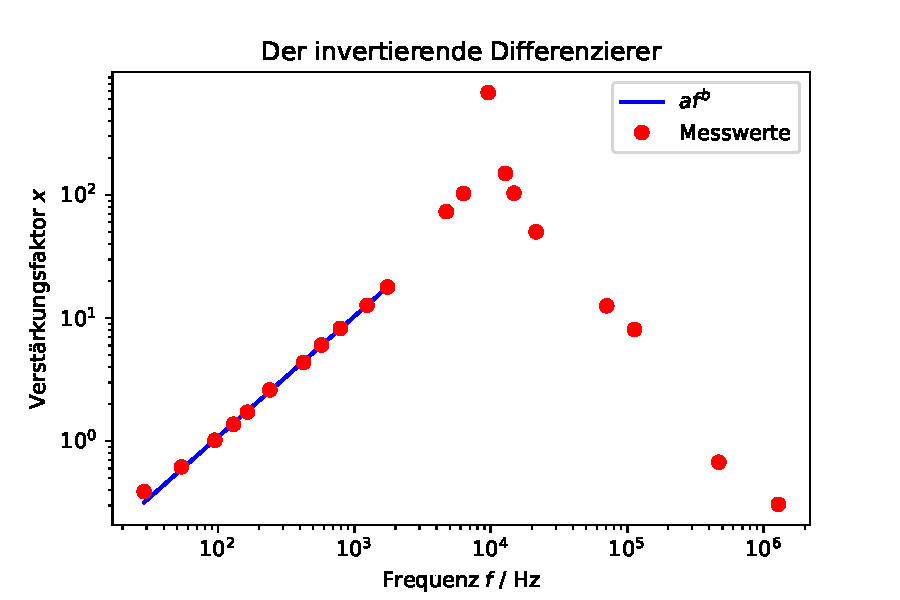
\includegraphics{content/grafiken/invdifferenzierer.pdf}
    \caption{Verstärkungskurve des invertierenden Differenzierers nach Eingangsfrequenz.}
    \label{fig:invdifferenzierer}
  \end{figure}

  \begin{figure}
    \centering
    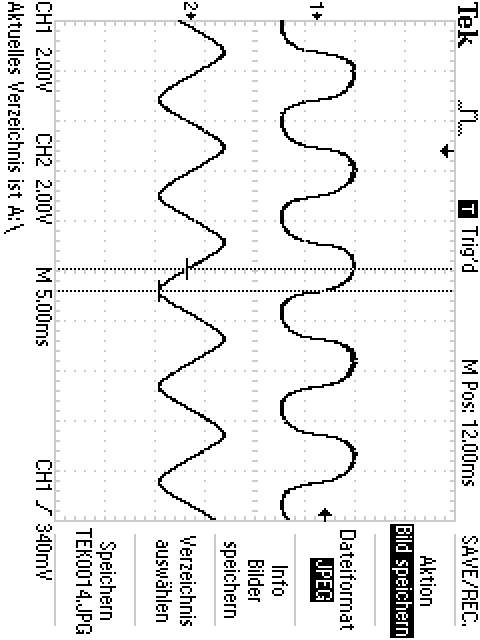
\includegraphics[width=0.3\textwidth,angle=90]{content/grafiken/invertierenderDifferenzierer/TEK0014.JPG}
    \caption{Oszilloskopbeild des invertierenden Differenzierers bei einer sinusförmigen Eingangsspannung.}
    \label{fig:sinusII}
  \end{figure}
  \begin{figure}
    \centering
    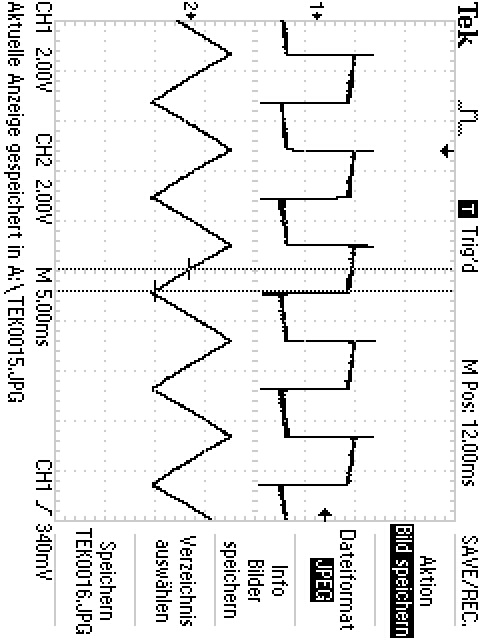
\includegraphics[width=0.3\textwidth,angle=90]{content/grafiken/invertierenderDifferenzierer/TEK0016.JPG}
    \caption{Oszilloskopbeild des invertierenden Differenzierers bei einer dreieckförmigen Eingangsspannung.}
    \label{fig:dreieckII}
  \end{figure}
  \begin{figure}
    \centering
    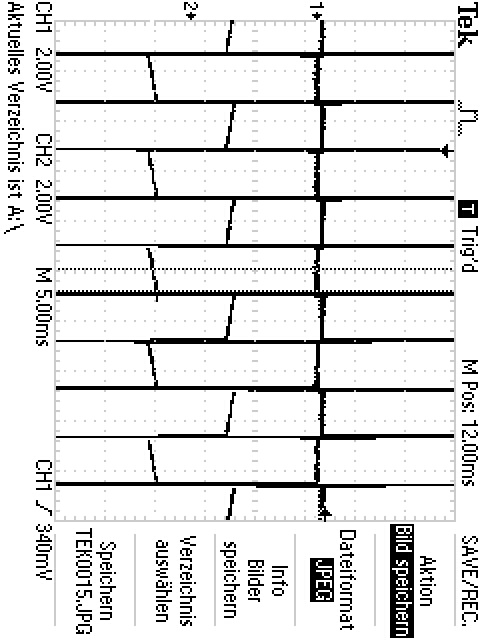
\includegraphics[width=0.3\textwidth,angle=90]{content/grafiken/invertierenderDifferenzierer/TEK0015.JPG}
    \caption{Oszilloskopbeild des invertierenden Differenzierers bei einer rechteckförmigen Eingangsspannung.}
    \label{fig:rechteckII}
  \end{figure}
  Beim Differentiator wird die Ableitung des Eingangssignal erwartet während beim Integrator die Stammfunktion 
  des Eingangssignals erwartet wird. Dies wird erfüllt.


  \subsection{Nicht-invertierender-Schmitt-Trigger}
  Zur Realisierung des Schmitttriggers wurde eine Schaltung nach \autoref{fig:SPschmitttrigger} mit 
  drei Verschiedenen Widerstandsverhältnissen aufgebaut und jeweils der Kippunkt an welchem die Schaltung
  durchschaltet bestimmt. In \autoref{fig:schmitttrigger} ist das Oszilloskopbild der Schaltung an dem Punkt dargestellt 
  an dem die Spannung grade die Schwelle überschreitet. Hieraus können die Kippspannungen abgelesen werden.
  Sie sind zusammen mit den Widerstandsverhältnissen in \autoref{tab:Schmitttrigger} dargestellt.
\label{sec:schmitt}
\begin{figure}
    \centering
    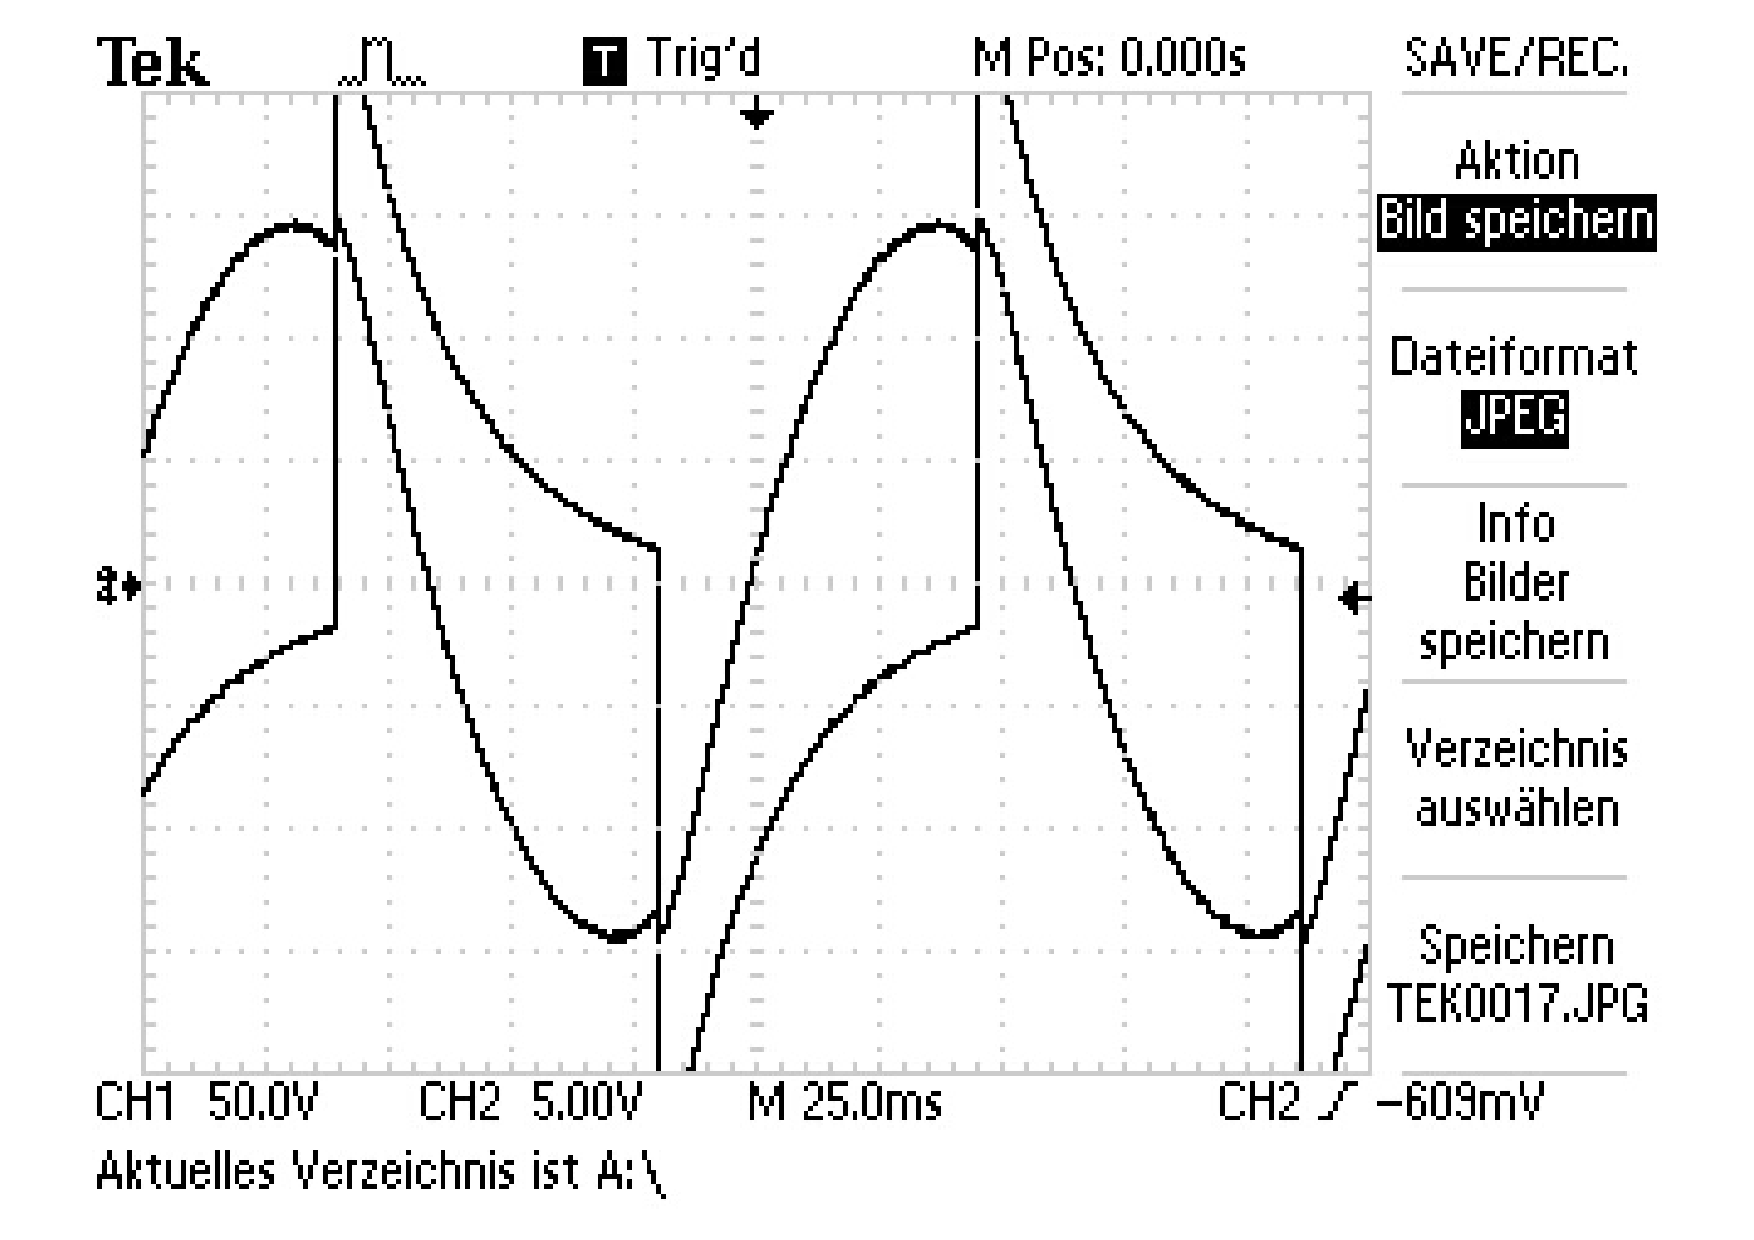
\includegraphics[width=1\textwidth]{content/grafiken/schmittTrigger/TEK0017.pdf}
    \caption{Oszilloskopbild des Spannungsverlaufs am invertierenden Schmitttrigger.}
    \label{fig:schmitttrigger}
  \end{figure}

  \begin{table}
    \centering
      \caption{In der Tabelle sind die theoretischen und experimentellen Kippspannungen und die Wiederstandsverhältnisse zu sehen.}
      \label{tab:Schmitttrigger}
      \sisetup{table-format=1.2}
      \begin{tabular}{S[table-format=3.2] S S S S S S S S [table-format=3.2]}
        \toprule
        {$R_1$/[$\si[]{K\Omega}$]} & {$R_2$/[$\si[]{K\Omega}$]}&{$U_{kipp,exp}$/[$\si[]{V}$]} &{$U_{kipp,theo}$/[$\si[]{V}$]}\\
        \midrule
        1 &  15 &{$$1.1$$}&{$$1$$}\\
        1 & 100 &{$$0.2$$}&{$$0.15$$}\\
        15 &100 &{$$1.35$$}&{$$2.25$$}\\
        
        \bottomrule
      \end{tabular}
    \end{table}
Die Kippunkte wurden mit einer Versorgungsspannung von $U_B$ über \autoref{eq:kipppunkt} berechnet.
























